\documentclass{article}

\usepackage{algorithm}
\usepackage[noend]{algpseudocode}
% latex math commands
% Vladimir Feinberg
% \vx notation for vectors from Goodfellow
% https://github.com/goodfeli/dlbook_exercises

% alphabet templates
% abcdefghijklmnopqrstuvwxyz
% ABCDEFGHIJKLMNOPQRSTUVWXYZ

% fonts, math, and layout commands
\usepackage{lmodern}
\usepackage{fullpage}
\usepackage{bbm}
\usepackage{enumerate}
\usepackage{amsmath}
\usepackage{amsthm}
\usepackage{amssymb}
\usepackage{amsfonts}
\usepackage{mathrsfs}
\usepackage{mathtools}
\usepackage[all]{xy}
\usepackage{algorithm}
\usepackage[noend]{algpseudocode}

% include graphics with \includegraphics
\usepackage{graphicx}
\usepackage{caption}

% \nicefrac{x}{y} gives a diagonal fraction bar x/y
\usepackage{nicefrac}

% \nurl{<url>}{link name} renders a blue underlined link
\usepackage[hidelinks]{hyperref}
\usepackage{xcolor}
\usepackage{url}
\newcommand{\nurl}[2]{\href{ #1 }{\color{blue}\underline{#2}}}

% brackets, norms, cardinalities
\newcommand{\pa}[1]{ \left({#1}\right) }
\newcommand{\ha}[1]{ \left[{#1}\right] }
\newcommand{\ca}[1]{ \left\{{#1}\right\} }
\newcommand{\inner}[1]{\left\langle #1 \right\rangle}
\newcommand{\innercpy}[1]{\inner{ #1, #1 }}
\newcommand{\norm}[1]{\left\lVert #1 \right\rVert}
\newcommand{\card}[1]{\left\lvert{#1}\right\rvert}
\newcommand{\abs}[1]{\card{#1}}

% math vectors
\newcommand{\va}{\textbf{a}}
\newcommand{\vb}{\textbf{b}}
\newcommand{\vc}{\textbf{c}}
\newcommand{\vd}{\textbf{d}}
\newcommand{\ve}{\textbf{e}}
\newcommand{\vf}{\textbf{f}}
\newcommand{\vg}{\textbf{g}}
\newcommand{\vh}{\textbf{h}}
\newcommand{\vi}{\textbf{i}}
\newcommand{\vj}{\textbf{j}}
\newcommand{\vk}{\textbf{k}}
\newcommand{\vl}{\textbf{l}}
\newcommand{\vm}{\textbf{m}}
\newcommand{\vn}{\textbf{n}}
\newcommand{\vo}{\textbf{o}}
\newcommand{\vp}{\textbf{p}}
\newcommand{\vq}{\textbf{q}}
\newcommand{\vr}{\textbf{r}}
\newcommand{\vs}{\textbf{s}}
\newcommand{\vt}{\textbf{t}}
\newcommand{\vu}{\textbf{u}}
\newcommand{\vv}{\textbf{v}}
\newcommand{\vw}{\textbf{w}}
\newcommand{\vx}{\textbf{x}}
\newcommand{\vy}{\textbf{y}}
\newcommand{\vz}{\textbf{z}}
\newcommand{\vzero}{\textbf{0}}
\newcommand{\vone}{\textbf{1}} 
\newcommand{\valpha}{{\boldsymbol\alpha}}
\newcommand{\vepsilon}{{\boldsymbol\epsilon}}
\newcommand{\veta}{{\boldsymbol\eta}}
\newcommand{\vsigma}{ {\boldsymbol\sigma}}
\newcommand{\vtheta}{ {\boldsymbol\theta}}
\newcommand{\vdelta}{ {\boldsymbol\delta}}
\newcommand{\vlambda}{ {\boldsymbol\lambda}}
\newcommand{\vmu}{ {\boldsymbol\mu}}
\newcommand{\vvartheta}{ {\boldsymbol\vartheta}}
\newcommand{\vbeta}{ {\boldsymbol\beta}}
\newcommand{\vphi}{ {\boldsymbol\phi}}


% math function arrows, misc binary math ops
\newcommand{\bij}{\leftrightarrow}
\newcommand{\inj}{\rightarrowtail}
\newcommand{\sur}{\twoheadedrightarrow}
\newcommand{\eqd}{\mathrel{\overset{\Delta}{=}}}

% common math sets
\newcommand{\Z}{\mathbb{Z}}
\newcommand{\R}{\mathbb{R}}
\newcommand{\C}{\mathbb{C}}
\newcommand{\N}{\mathbb{N}}
\newcommand{\Q}{\mathbb{Q}}
\newcommand{\F}{\mathbb{F}}
\newcommand{\T}{\mathbb{T}}

% limits
\def\sumn{\sum_{n=0}^\infty}
\def\limn{\lim_{n\rightarrow\infty}}
\def\prodn{\prod_{n=0}^\infty}

% mathcal
\newcommand{\mcA}{\mathcal{A}}
\newcommand{\mcB}{\mathcal{B}}
\newcommand{\mcC}{\mathcal{C}}
\newcommand{\mcD}{\mathcal{D}}
\newcommand{\mcE}{\mathcal{E}}
\newcommand{\mcF}{\mathcal{F}}
\newcommand{\mcG}{\mathcal{G}}
\newcommand{\mcH}{\mathcal{H}}
\newcommand{\mcI}{\mathcal{I}}
\newcommand{\mcJ}{\mathcal{J}}
\newcommand{\mcK}{\mathcal{K}}
\newcommand{\mcL}{\mathcal{L}}
\newcommand{\mcM}{\mathcal{M}}
\newcommand{\mcN}{\mathcal{N}}
\newcommand{\mcO}{\mathcal{O}}
\newcommand{\mcP}{\mathcal{P}}
\newcommand{\mcQ}{\mathcal{Q}}
\newcommand{\mcR}{\mathcal{R}}
\newcommand{\mcS}{\mathcal{S}}
\newcommand{\mcT}{\mathcal{T}}
\newcommand{\mcU}{\mathcal{U}}
\newcommand{\mcV}{\mathcal{V}}
\newcommand{\mcW}{\mathcal{W}}
\newcommand{\mcX}{\mathcal{X}}
\newcommand{\mcY}{\mathcal{Y}}
\newcommand{\mcZ}{\mathcal{Z}}

% measure theory
\newcommand{\indicator}{\mathbbm{1}}
\DeclareMathOperator{\Laplace}{Laplace}
\DeclareMathOperator{\Poisson}{Poisson}
\DeclareMathOperator{\Exponential}{Exponential}
\DeclareMathOperator{\Multinomial}{Multinomial}
\DeclareMathOperator{\Bernoulli}{Bernoulli}
\DeclareMathOperator{\Categorical}{Categorical}
\DeclareMathOperator{\Uniform}{Uniform}
\DeclareMathOperator{\Binomial}{Binomial}
\DeclareMathOperator{\Hypergeometric}{Hypergeometric}
\DeclareMathOperator{\GammaDist}{Gamma}
\DeclareMathOperator{\NegativeBinomial}{NegativeBinomial}
\DeclareMathOperator\mathProb{\mathbb{P}}
\renewcommand{\d}[1]{\mathop{\mathrm{d} #1 }}
\DeclarePairedDelimiterX{\infdivx}[2]{(}{)}{ #1\;\delimsize\|\;#2 }
\newcommand{\dkl}[2]{\mathop{D_\text{KL}}\infdivx{#1}{#2}}

% distributions
\makeatletter
\newcommand{\distas}[1]{\mathbin{\overset{#1}{\kern\z@\sim}}}%
\makeatother
\newcommand{\disteq}{\overset{d}{=}}
\newcommand{\distiid}{\distas{\text{iid}}}
\newcommand\independent{\protect\mathpalette{\protect\independenT}{\perp}}
\def\independenT#1#2{\mathrel{\rlap{$#1#2$}\mkern2mu{#1#2}}}
\newcommand{\convdist}{\mathbin{\overset{\text{d}}{\longrightarrow}}}
\newcommand{\convas}{\mathbin{\overset{\text{as}}{\longrightarrow}}}
\newcommand{\convpb}{\mathbin{\overset{\text{pb}}{\longrightarrow}}}

\renewcommand{\P}{\mathProb} % need to overwrite stupid paragraph symbol
\DeclareMathOperator\mathExp{\mathbb{E}}
\DeclareMathOperator*\mathExpUnder{\mathbb{E}}
\newcommand{\E}{\mathExp}

\newcommand{\sa}{{$\sigma$-algebra}}
\newcommand{\OR}{{\overline{\R}}}
\newcommand{\OX}{{\overline{X}}}
\DeclareMathOperator{\power}{{\mathcal{P}}}
\DeclareMathOperator{\var}{var}
\DeclareMathOperator{\cov}{cov}

% \set{from set}{condition} with set-builder notation
% conditional expectation is analogous
\newcommand{\set}[2]{ \left\{ #1 \,\middle|\, #2 \right\} }
\newcommand{\CE}[2]{ \mathExp\left[ #1 \,\middle|\, #2 \right] }

% linear-algebra related
\newcommand{\mat}[1]{\begin{pmatrix} #1 \end{pmatrix}}
\newcommand{\detmat}[1]{\begin{vmatrix} #1 \end{vmatrix}}
\DeclareMathOperator{\spanb}{span}
\DeclareMathOperator{\conv}{conv} % convex hull
\DeclareMathOperator{\cone}{cone}
\DeclareMathOperator{\vectorize}{vec}
\DeclareMathOperator{\matricize}{mat}
\DeclareMathOperator{\adj}{adj}
\DeclareMathOperator{\diag}{diag}
\DeclareMathOperator{\tr}{tr}
\DeclareMathOperator{\rank}{rank}
\DeclareMathOperator*{\argmin}{argmin}
\DeclareMathOperator*{\argmax}{argmax}
\DeclareMathOperator*{\proj}{proj}

% complex analysis
\DeclareMathOperator{\MyRe}{Re}
\DeclareMathOperator{\MyIm}{Im}
\DeclareMathOperator{\image}{image}
\DeclareMathOperator{\supp}{supp}

% typical numerical operators
\DeclareMathOperator{\sgn}{sgn}

% graphs
\DeclareMathOperator{\diam}{diam}

% constants
\renewcommand{\d}[1]{\mathop{\mathrm{d} #1 }}
\newcommand{\e}{\mathrm{e}}
\renewcommand{\i}{\imath}

% \bigtimes: large indexed cross product
\makeatletter
\DeclareFontFamily{U}  {MnSymbolF}{}
\DeclareSymbolFont{symbolsMN}{U}{MnSymbolF}{m}{n}
\SetSymbolFont{symbolsMN}{bold}{U}{MnSymbolF}{b}{n}
\DeclareFontShape{U}{MnSymbolF}{m}{n}{
    <-6>  MnSymbolF5
   <6-7>  MnSymbolF6
   <7-8>  MnSymbolF7
   <8-9>  MnSymbolF8
   <9-10> MnSymbolF9
  <10-12> MnSymbolF10
  <12->   MnSymbolF12}{}
\DeclareFontShape{U}{MnSymbolF}{b}{n}{
    <-6>  MnSymbolF-Bold5
   <6-7>  MnSymbolF-Bold6
   <7-8>  MnSymbolF-Bold7
   <8-9>  MnSymbolF-Bold8
   <9-10> MnSymbolF-Bold9
  <10-12> MnSymbolF-Bold10
  <12->   MnSymbolF-Bold12}{}
\DeclareMathSymbol{\tbigtimes}{\mathop}{symbolsMN}{2}
\newcommand*{\bigtimes}{%
  \DOTSB
  \tbigtimes
  \slimits@ 
}
\makeatother

% category theory arguments
% See https://tex.stackexchange.com/questions/356873
\newcommand{\catfst}{{-}}
\newcommand{\catsnd}{{=}}
\newcommand{\cattrd}{{\equiv}}
\DeclareMathOperator{\Id}{Id}
\newcommand{\opcat}[1]{{#1}^{\text{op}}}
\DeclareMathOperator{\Hom}{hom}
\DeclareMathOperator{\Ob}{ob}
\DeclareMathOperator{\El}{el}
\DeclareMathOperator{\colim}{colim}
\DeclareMathOperator{\Sym}{Sym}

% references
\newcommand{\figref}[1]{Figure~\ref{fig:#1}}
\newcommand{\tabref}[1]{Table~\ref{tab:#1}}
\newcommand{\secref}[1]{Section~\ref{sec:#1}}
\newcommand{\equref}[1]{Equation~\ref{eq:#1}}
\renewcommand{\algref}[1]{Algorithm~\ref{alg:#1}}

% centered figure with \autofig{filepath}{\label{fig:somelabel}}{caption}
\newcommand{\autofig}[3]{
  \begin{figure}[!ht]
    \begin{center}
      \includegraphics[width=0.8\columnwidth]{#1}
    \end{center}
    \caption{#3}
    #2
\end{figure}
}

\usepackage{subcaption}


\title{Constrained Model Predictive Control for Learned Dynamics\\\large CS 294-112}
\author{Vladimir Feinberg, Samvit Jain, Michael Whittaker}
\date{1 December 2017}

\begin{document}

\maketitle

\section{Abstract}

Deep reinforcement learning has recently made progress in traditionally unsolvable problems for continuous control. Such continuous control problems are characterized by a MDP setting, where an agent interacts with the world, characterized by a set of states $\mcS$, by taking actions chosen from a set of actions $\mcA$ to maximize the expected net present value of a reward given over time. Episodes of a single problem share the same MDP setting, but differ in the initial state. We are interested in spaces where the dimension of $\mcA$ is moderately large, continuous, or both; adversarial and stochastic worst-case or high-probability methods are not applicable.

We consider a model-based method, Model Predictive Control (MPC), with unknown dynamics. In other words, both the transition model and policy for an unknown MDP must be learned, only by interacting with the environment. We find that even for simple continuous control problems, dynamics learning can be difficult. The usual MPC algorithm, which seeks to optimize over any actions and states over a small horizon, exhibits pathological behavior even for short horizons with poor dynamics due to a blunt optimization approach.

We show that the root of the pathological behavior with unconstrained MPC derives from over-optimism during the planning phase. As an MPC agent improves its planning using a trained dynamics model, the agent actually tends to perform worse when using the real dynamics. In particular, the objective value of the reward function at the end of the planning phase can be viewed as the planner's estimator for future rewards. Treating it this way we find that this value over-inflates as the MPC planning optimization quality improves.

We handicap MPC planning by only allowing optimization along the first action, so while planning may account for future steps in the simulated horizon, no new actions can be taken. This handicapped optimization performs uniformly better on a variety of small continuous control tasks.

By taking into account, even crudely, for some uncertainty in the dynamics model, we can improve MPC performance. This indicates that a more careful approach which carefully analyzes dynamics uncertainty may be a promising direction for future work.

\section{Introduction}
Model-free reinforcement learning algorithms directly learn a policy that maps a state to the action that, when taken, maximizes the expected reward returned by the environment. Model-free methods perform all planning \emph{implicitly} and only with state information. Model-based reinforcement learning algorithms, on the other hand, construct models of the environment's dynamics and use the models to \emph{explicitly} plan. These model-based methods tend to have improved sample complexities relative to their model-free counterparts.

However, constructing a model of the world---even in its restricted form as a simple dynamics prediction problem in continuous control---complicates the existing deep RL architecture. Purely model-based methods assume they have a completely accurate dynamics model and optimize expected reward under this assumption. Understandably, such methods are inherently limited by how accurate the dynamics model is. For instance, one such pure model-based algorithm, iLQG, was outperformed by an algorithm which used a learned model, Guided Policy Search~\cite{levine2014learning}. Moreover, generic global models, such as neural networks, have not historically performed as well as simple, local linear models~\cite{gu2016continuous}.  Altogether, pure model-based methods are fundamentally limited by \emph{model bias} and pure model-free methods are fundamentally limited by \emph{policy variance}.

As is common in machine learning, we need to find the right trade-off between bias and variance. One way to bridge this gap is to explicitly include model-predicted rewards in the value estimates. In the style of SVG \cite{heess2015learning}, we might accelerate value learning by mixing in a model-based expansion of our value estimates, where the value $V^\pi:\mcS\rightarrow \R$ (the true net present value for the reward at a given state) is approximated with the help of dynamics $f:\mcS\times \mcA\rightarrow \mcS$ describing transitions deterministically for simplicity and the reward $r:\mcS\times\mcA\times\mcS\rightarrow\R$ for a policy $\pi:\mcS\rightarrow \mcA$:
$$
  V^\pi(s_1)
    \approx \pa{\sum_{t=1}^H r(s_t,a_t,s_{t+1})} + \hat{V}(s_{H+1});
    \quad s_{t+1} \triangleq f(s_t, a_t), a_t\triangleq \pi(s_t)
$$
While a viable approach, an implementation must take care to account for bias in $f$, which may skew estimates in $V$, no matter how good $\hat V$ is. Second, this introduces a nuanced coupling of the training of $f,\hat V,\pi$ at the same time.

\section{Background}
We investigate a use of dynamics models that is presumably less-coupled with policy learning. We will revisit the potential for fused model-free and model-based methods at the end of the report. MPC chooses actions using an open-loop planner $P$ that accepts a dynamics model $f$ and a horizon $H$ and returns the next $H$ actions to play. MPC iteratively queries the planner at each time step, playing only the first action in the plan (\algref{mpc}).

\begin{algorithm}
\caption{The \textsc{MPC} algorithm acts as a policy, returning an action for a given state, using an internal planner and a dynamics model.} \label{alg:mpc}
\begin{algorithmic}[1]
\Procedure{MPC}{state $s$, horizon $H$, reward $r$, dynamics $f$, planner $P$}
\State $\ca{a_t}_{t=1}^H=P(s, H, r, f)$
\State\Return $a_1$
\EndProcedure
\end{algorithmic}
\end{algorithm}

Most planners treat $f$ as the true dynamics and attempt to solve the following maximization, which is frequently intractable:
\begin{align}
    \max_{\{a_t,s_t\}_{t=1}^H}&\;\;\;\; \sum_{t=1}^H r(s_t, a_t) \label{eq:unconstrained}\\
    \text{s.t.} &\;\;\;\; s_{t+1} = f(s_t,a_t)\nonumber
\end{align}

A typical way of estimating a solution to \equref{unconstrained} is with the random shooter method, which samples the $t$-th action from the distribution $A_t(s_t)$ (\algref{rs}).

\begin{algorithm}
\caption{The \textsc{RandomShooter} algorithm is a planner that approximately solves \equref{unconstrained}, where the quality of the approximation improves with the number of trials it attempts. Altogether, \textsc{RandomShooter} is a stochastic policy available only in this generative form, returning an action $a$ for a provided state $s$. The \textsc{RandomShooter}'s properties highly depend on the state-conditional time-dependent action sampling distributions $A_t$.}\label{alg:rs}
\begin{algorithmic}[1]
\Procedure{RandomShooter}{state $s$, horizon $H$, reward $r$, dynamics $f$, samplers $\ca{A_t}_{t=1}^H$}
\State $\ca{s_1^{(i)}\gets s}_{i=1}^K$.
\For { $i\gets 1, \ldots, K$}
\For { $t\gets 1,\ldots,H$}
\State sample $a_t^{(i)}\sim A_t(s_t)$
\State $s_{t+1}^{(i)}\gets f\pa{s_t^{(i)},a_t^{(i)}}$
\EndFor
\State $R_i\gets\sum_{t=1}^{H}r\pa{s_{t}^{(i)},a_t^{(i)},s_{t+1}^{(i)}}$
\EndFor
\State $i_*=\argmax_i R_i$
\State \Return $\ca{s^{(i*)}_t}_{t=1}^H$ % The planner above returned the whole action sequence, not just the first one.
\EndProcedure
\end{algorithmic}
\end{algorithm}

We believe \textsc{RandomShooter}, or more generally any solution to \equref{unconstrained}, works well when the corresponding reward $R_i$ is a decent estimator for the true $H$-step reward of the agent. It is important to note that the agent takes $a_1^{(i_*)}$ now and continues with \textsc{MPC} later, so there will necessarily be some mismatch. In fact, one might expect positive bias, since the true reward comes from planning $H$ steps ahead for each of the agent's next $H$ steps, looking ahead $2H$ timesteps, as opposed to their initial estimate of its reward through \algref{rs}, which only looks $H$ steps ahead.

Assuming a good reward estimator $R_i$, choosing the first action $a_1^{(i_*)}$ that results in the best $R_i$ would be the smartest move one could make. Usually, one specifies $A_t(s)=\Uniform \mcA$ for a rectangle $\mcA$, independent of $t,s$ (Uniform RS MPC). But a uniform distribution is a poor representation of future \textsc{MPC} steps: it stands to reason that a more intelligent selection of $A_t$ might improve performance.

\section{Contributions}

We find that one needs to be concerned with both underoptimizing and overoptimizing \equref{unconstrained}. In particular, because $f$ is learned and partially inaccurate, improvements in \equref{unconstrained} do not correspond to improvements in actual reward. For instance, letting $\tilde R$ be the true $H$-step reward, the reward predicted by \algref{rs} with Uniform RS MPC, $\tilde R - R_{i_*}$, becomes increasingly negative as optimization quality is improved. As a function of optimization quality, the reward curve is actually U-shaped: too little optimization, and poor actions are chosen. Too much, and bias prevents or hurts improvement. Given our findings, we present a new MPC objective as an alternative to \equref{unconstrained} and propose several methods to investigate in future work.

\section{Method}

We propose learning a stationary action distribution conditional on the state, $\pi_\theta(s)$. This policy is used to regularize the MPC optimization. In particular, if the planner is \textsc{RandomShooter}, then we select $A_t^{(\pi_\theta)}$ to be a distribution that is some function of $\pi_\theta$. Overall, we consider a joint training algorithm, \algref{train}.

\begin{algorithm}
\caption{This algorithm assumes that we have the testing environment with which we may perform real rollouts to learn from. We consider some fixed class of deterministic functions $F$ to model dynamics, and a parameterization $\pi_\theta$ of generative action distributions conditioned on states, coupled with an associated loss $J$.} \label{alg:train}
\begin{algorithmic}[1]
\Procedure{TrainMPC}{iterations $N$, starter transition dataset $\mcD$, reward $r$}
\For { $i\gets 1, \ldots, N$}
\State $f\gets \argmin_{f \in F}\E\ha{\norm{f(s,a)-s'}^2}$, where $(s,a,s')\sim\Uniform\mcD$
\State $\theta \gets \argmin_\theta J(\theta, \mcD)$
\State sample $E$ episodes $\mcD'$ of $\textsc{MPC}(\cdot,  H, r, f, P_\theta)$, where $P_\theta$ is some planner parameterized by $\theta$.
\State $\mcD\gets\mcD'\cup\mcD$
\EndFor
\State \Return $\textsc{MPC}(\cdot,  H, r, f, P_\theta)$
\EndProcedure
\end{algorithmic}
\end{algorithm}

Since the dynamics are learned from historical data, we propose a planner that optimizes \equref{constrained}, where $\mcF_t$ is a region where we consider our dynamics model to be accurate.

\begin{align}
    \max_{\{a_t,s_t\}_{t=1}^H}&\;\;\;\; \sum_{t=1}^H r(s_t, a_t) \label{eq:constrained}\\
  \text{s.t.} &\;\;\;\; s_{t+1} = f(s_t,a_t)\nonumber\\
      & \;\;\;\;(a_t,s_t)\in \mcF_t \nonumber
\end{align}

For instance, we might claim that our dynamics model is accurate for actions and states within some $\epsilon$-ball of historical action and state distributions. In other words, let $J$ be the cost for fitting a state-conditional action distribution $\pi_\theta$ on our historical data $\mcD$. Then we might define $\mcF_t\triangleq B_{\epsilon_t}(\pi_\theta(s_t))\times B_{\epsilon_t'}(\bar s_t)$, where $\bar s_{t+1}=f(\bar s_t, \pi_\theta (\bar s_t))$: actions must be near a historical mean of actions taken in the corresponding state and states must be near the states that would come from a historical trajectory. $B_r(z)$ indicates a ball of radius $r$ around $z$.

An approximate way of optimizing the above objective for $\epsilon_1=\infty$ and $\epsilon_t,\epsilon_t'=0$ otherwise would be to only allow \textsc{RandomShooter} to sample randomly on the first action, and otherwise stick to a policy representative of past actions (\equref{delta}). In general, setting the support of the sampling distributions for \textsc{RandomShooter} results in Monte Carlo optimization of the constrained problem.
\begin{equation}\label{eq:delta}
  \begin{gathered}
  A_t(s)=\begin{cases}
\Uniform\pa{\mcA}    & t=1 \\
\pi_\theta(s)\triangleq\delta_{g_\theta(s)} & \text{otherwise}
\end{cases} \\
J(\theta,\mcD)=\E_{(s,a)\sim \mcD}\norm{a-A}^2=\E_{(s,a)\sim \mcD}\norm{a-g_\theta(s)}^2;\;A\sim\delta_{g_\theta(s)}
\end{gathered}
\end{equation}
Above, $g$ is some function parameterized by $\theta$, such as a neural network.

We refer to \textsc{TrainMPC} with \textsc{RandomShooter} using the distributions of \equref{delta} as $\delta$ RS MPC. We also consider a simple, parameter-less regularization $g_\theta(s)=\vzero$, called $0$ RS MPC.

\section{Results}

% centered figure with \autofig{filepath}{\label{fig:somelabel}}{caption}

\subsection{Easy Cheetah}\label{sec:easy-cheetah}
For preliminary validation of our ideas, we consider the \texttt{HalfCheetah-v1} environment with the reward function provided in Homework 4: an environment we call easy cheetah. In particular, the reward function includes additional penalties for undesirable behavior, making this an easy baseline to test on.\footnote{Here our dynamics model is represented by a neural network of depth 2 and width 500. With an MPC horizon $H=15$ and $K=1000$ simulation paths, we evaluate the performance of the proposed methods over several iterations of the training procedure (\algref{train}). Every iteration takes 10 sample episodes, and trains the dynamics for 60 epochs with a $10^{-3}$ learning rate. The policy optimization step, if present, does 100 epochs with $10^{-3}$ learning rate on a neural network $g_\theta$ of depth 5 and width 32. The universal batch size was 512. Reported results are averages over 4 seeds.}

The performance of the various MPC policies is shown in \figref{easy-cheetah-return}. The underlying $\pi_\theta$ policy (henceforth the ``learner'') is poor (\figref{easy-cheetah-learner}), so the improvement it induces in MPC is likely coming from its regularizing properties rather than any smarter selection of actions that may be induced by the learner.
%
Notice that both regularized versions reduce the bias of the predicted reward from the MPC optimization, $\tilde R - R_i$ (\figref{easy-cheetah-bias}). This is not due to catastrophic cancellation either, as the MSE $(\tilde R - R_i)^2$ figures demonstrate (\figref{easy-cheetah-mse}).

\begin{figure}[!ht]
  \centering

  \begin{subfigure}[b]{0.48\columnwidth}
    \centering
    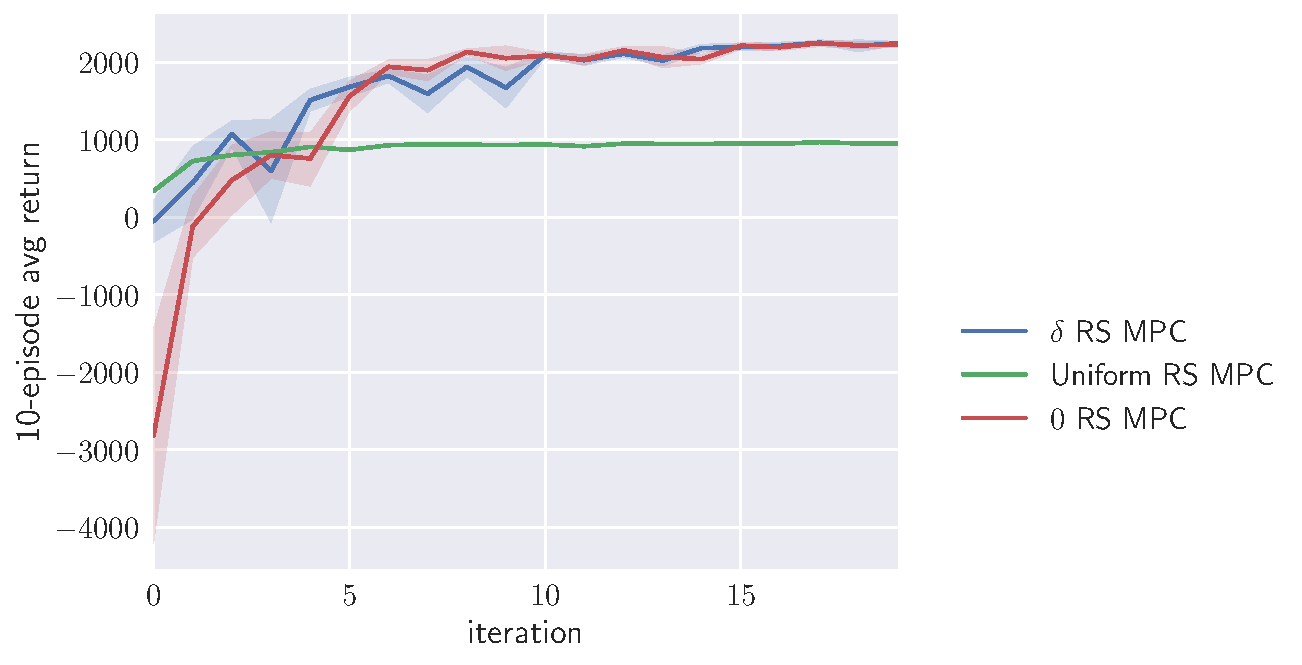
\includegraphics[width=\textwidth]{easy-cheetah-return.pdf}
    \caption{%
      Performance during the course of optimization in the easy cheetah
      setting. Note both regularized versions significantly outperform Uniform
      MPC.
    }\label{fig:easy-cheetah-return}
  \end{subfigure}\hspace{1em}
  \begin{subfigure}[b]{0.48\columnwidth}
    \centering
    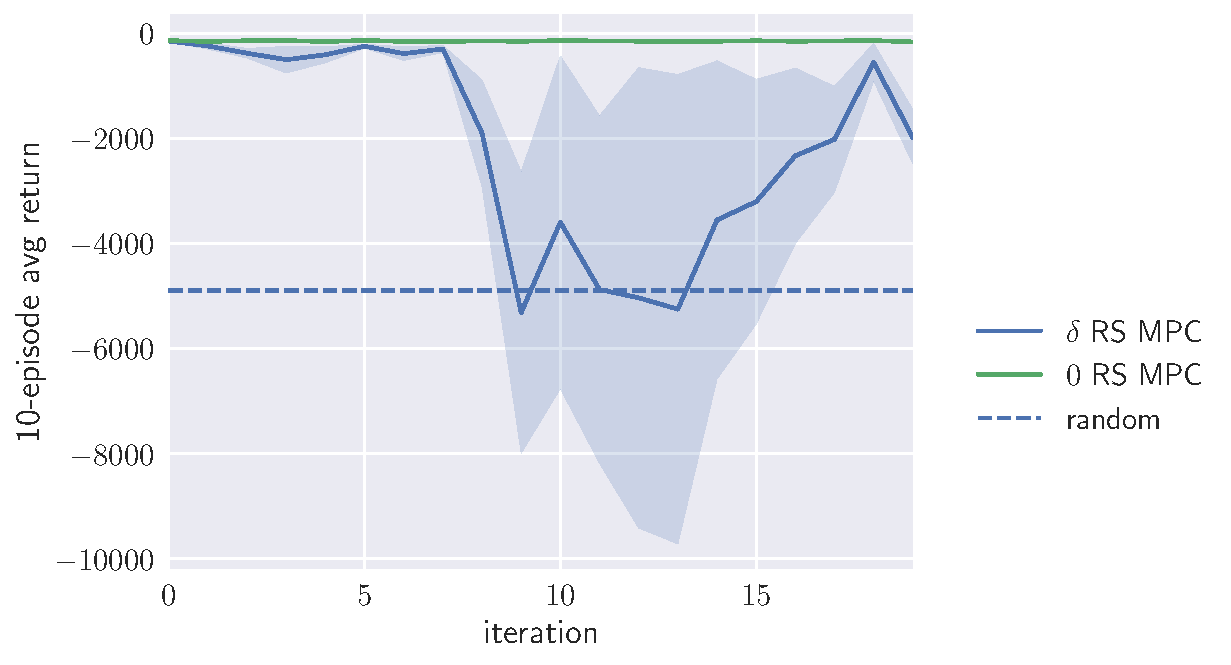
\includegraphics[width=\textwidth]{easy-cheetah-learner-return.pdf}
    \caption{%
      Performance of the underlying learner $\pi_\theta$ in the easy cheetah
      setting, during the course of optimization. We compare to the performance
      of an agent taking random actions uniformly on the action space.
    }\label{fig:easy-cheetah-learner}
  \end{subfigure}

  \vspace{1em}

  \begin{subfigure}[b]{0.48\columnwidth}
    \centering
    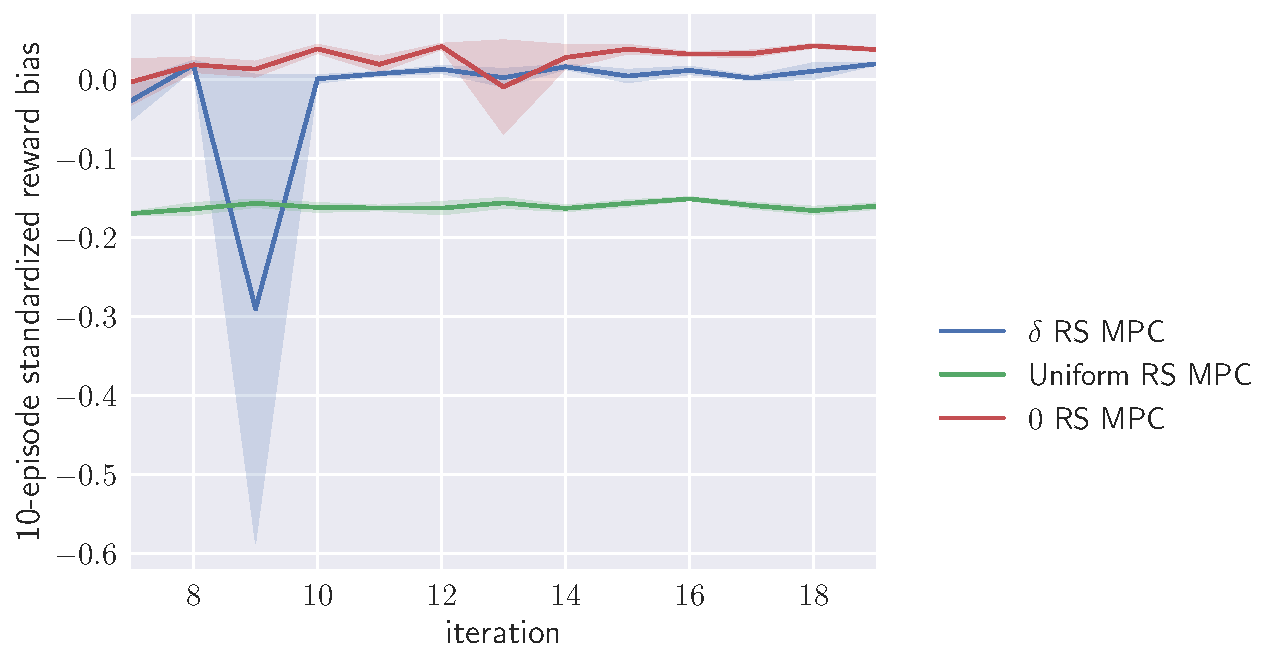
\includegraphics[width=\textwidth]{easy-cheetah-reward-bias.pdf}
    \caption{%
      Easy cheetah MPC predicted reward bias is calculated as the true $H$-step
      reward minus the MPC's planner objective value $H$ steps ago. A very
      negative value indicates overoptimism in the expected reward during MPC
      planning. We will refer to this as reward bias from this point.
    }\label{fig:easy-cheetah-bias}
  \end{subfigure}\hspace{1em}
  \begin{subfigure}[b]{0.48\columnwidth}
    \centering
    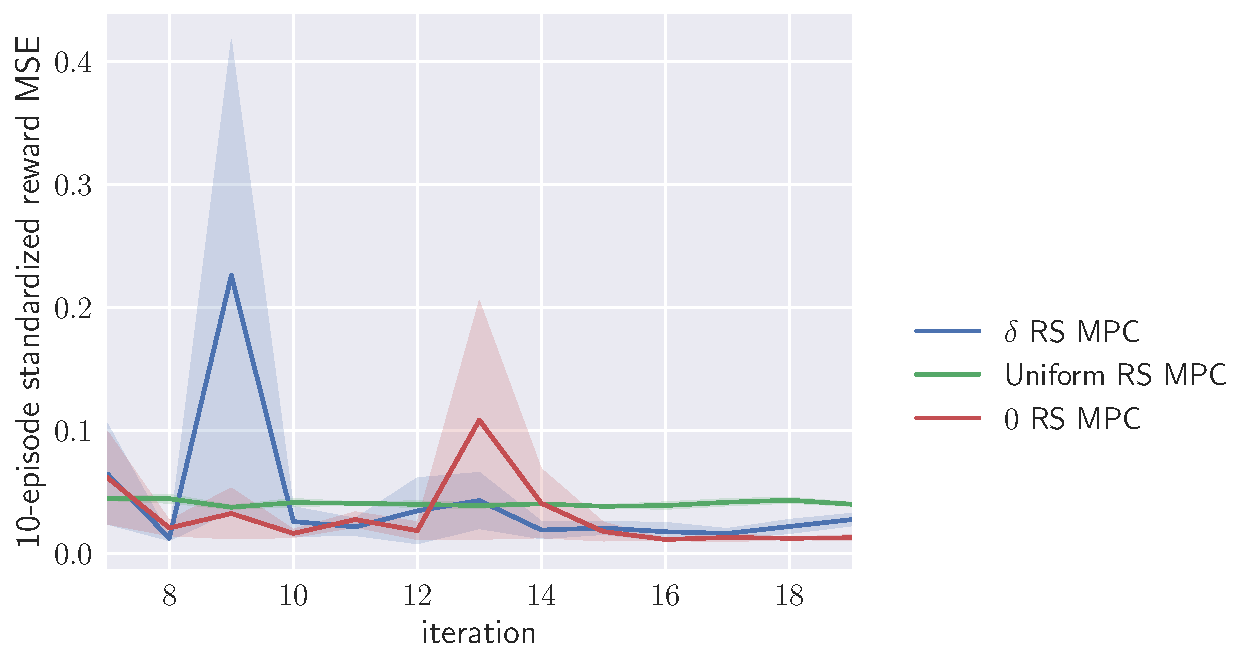
\includegraphics[width=\textwidth]{easy-cheetah-reward-mse.pdf}
    \caption{%
      Easy cheetah MPC predicted reward MSE. This is the average bias of
      \figref{easy-cheetah-bias}, squared.
    }\label{fig:easy-cheetah-mse}
  \end{subfigure}

  \caption{Easy cheetah experiments}
  \label{fig:easy-cheetah}
\end{figure}

% \autofig{easy-cheetah-return.pdf}{\label{fig:easy-cheetah-return}}{Performance during the course of optimization in the easy cheetah setting. Note both regularized versions significantly outperform Uniform MPC.}
% \autofig{easy-cheetah-learner-return.pdf}{\label{fig:easy-cheetah-learner}}{Performance of the underlying learner $\pi_\theta$ in the easy cheetah setting, during the course of optimization. We compare to the performance of an agent taking random actions uniformly on the action space.}
% \autofig{easy-cheetah-reward-bias.pdf}{\label{fig:easy-cheetah-bias}}{Easy cheetah MPC predicted reward bias is calculated as the true $H$-step reward minus the MPC's planner objective value $H$ steps ago. A very negative value indicates overoptimism in the expected reward during MPC planning. We will refer to this as reward bias from this point.}
% \autofig{easy-cheetah-reward-mse.pdf}{\label{fig:easy-cheetah-mse}}{Easy cheetah MPC predicted reward MSE. This is the average bias of \figref{easy-cheetah-bias}, squared.}

\section{Reward Bias}
We now investigate more carefully the over-optimization that occurs when MPC optimizes the unconstrained \equref{unconstrained}. We consider the usual \texttt{HalfCheetah-v1} environment.\footnote{We use a minor modification to the observations in this environment to include additional position information in the state so that the usual Half Cheetah reward function is a function of the transitions. Otherwise MPC optimization would be impossible because usually the Half Cheetah enviroment determines the reward based on a latent coordinate position.} In particular, we improve the quality of the \textsc{RandomShooter} optimization of \equref{unconstrained} in the Uniform RS MPC procedure by increasing $K$. We note that as $K$ increases, so does the over-optimism in the expected reward from the MPC objective (\figref{mpc-bias}, \figref{mpc-mse}). Note that the predicted reward is a function of the states projected by the MPC planner $\ca{s_t}_{t=1}^H$. Then, a mismatch in the reward function implies a mismatch in predicted states, because the state space topology is necessary finer than the pushforward topology on the state space induced by the (continuous) reward function. This may explain why increases in $K$ do not result in improvements in episode reward, and start to hamper performance for large $K$ (\figref{mpc-reward}).\footnote{Hyperparameters are as in \secref{easy-cheetah}, except for $K$ which is modified as indicated.}

\begin{figure}[!ht]
  \centering

  \begin{subfigure}[b]{0.48\columnwidth}
    \centering
    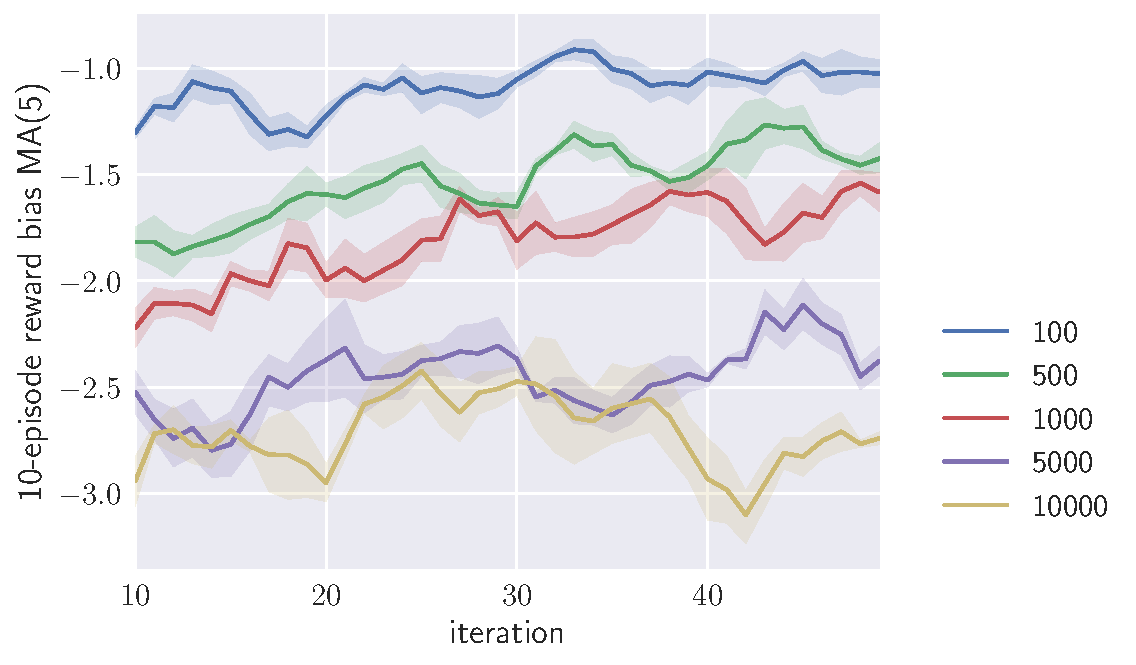
\includegraphics[width=\textwidth]{mpc-reward-bias.pdf}
    \caption{%
      Half Cheetah predicted reward bias for Uniform RS MPC on a variety of
      $K$, smoothed over the 5 previous iterations.
    }\label{fig:mpc-bias}
  \end{subfigure}\hspace{1em}
  \begin{subfigure}[b]{0.48\columnwidth}
    \centering
    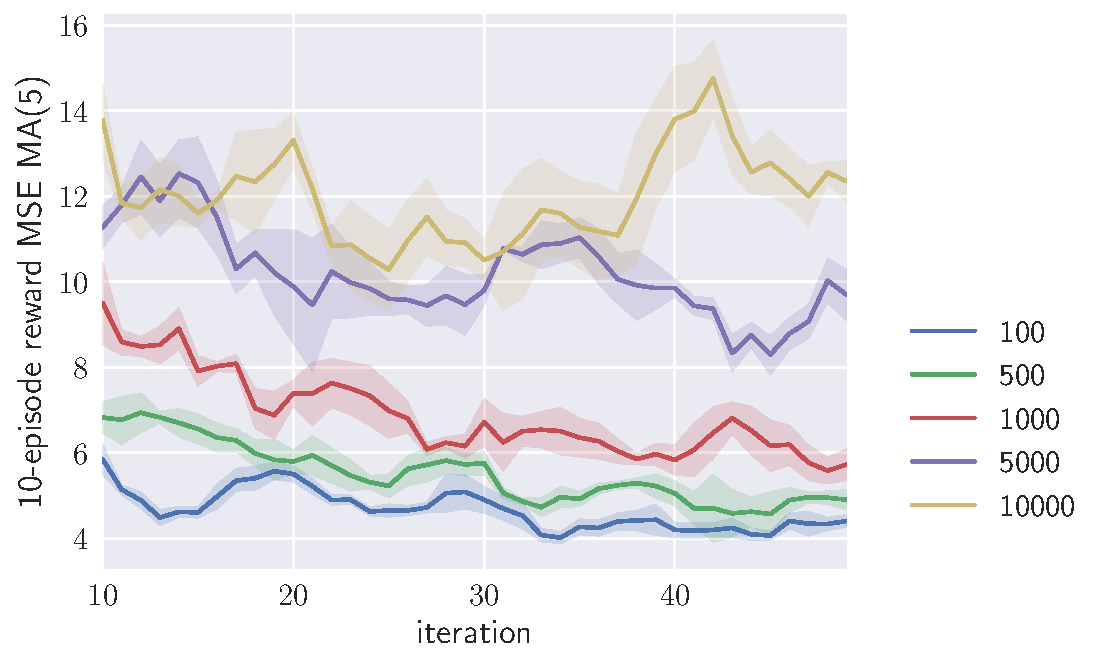
\includegraphics[width=\textwidth]{mpc-reward-mse.pdf}
    \caption{%
      Half Cheetah predicted reward MSE for Uniform RS MPC on a variety of $K$,
      smoothed.
    }\label{fig:mpc-mse}
  \end{subfigure}

  \vspace{1em}

  \begin{subfigure}[b]{0.48\columnwidth}
    \centering
    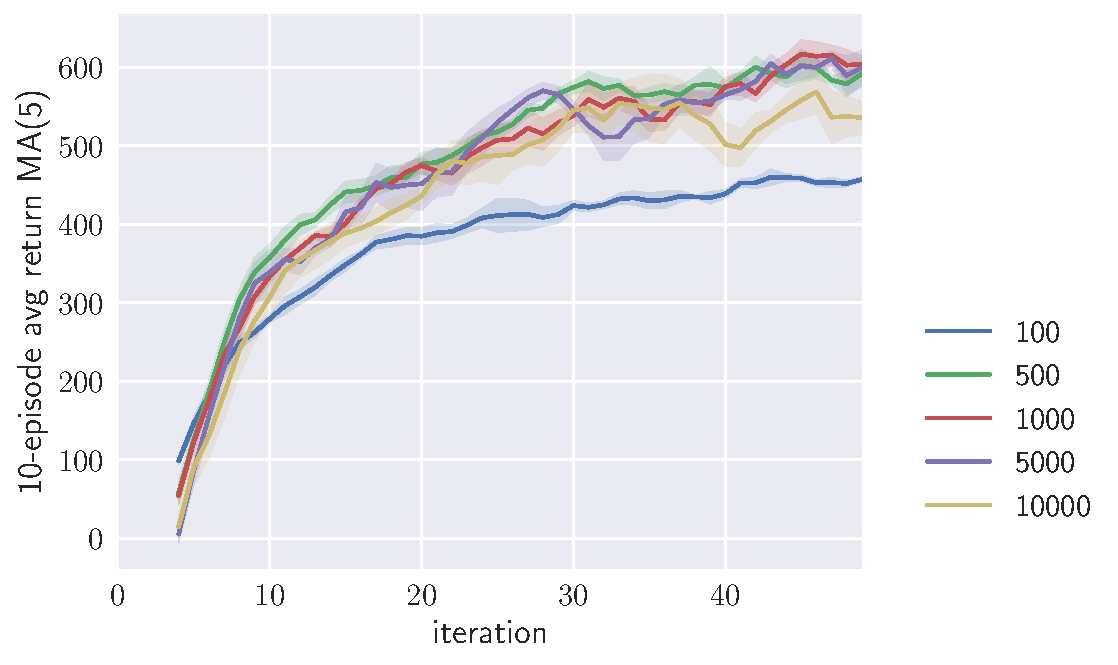
\includegraphics[width=\textwidth]{mpc-return.pdf}
    \caption{%
      Half Cheetah reward for Uniform RS MPC on a variety of $K$, smoothed.
      Note that both underoptimizing and overoptimizing reduces performance.
    }\label{fig:mpc-reward}
  \end{subfigure}

  \caption{\texttt{HalfCheetah-v1} experiments}
  \label{fig:half-cheetah}
\end{figure}

% \autofig{mpc-reward-bias.pdf}{\label{fig:mpc-bias}}{Half Cheetah predicted reward bias for Uniform RS MPC on a variety of $K$, smoothed over the 5 previous iterations.}
% \autofig{mpc-reward-mse.pdf}{\label{fig:mpc-mse}}{Half Cheetah predicted reward MSE for Uniform RS MPC on a variety of $K$, smoothed.}
% \autofig{mpc-return.pdf}{\label{fig:mpc-reward}}{Half Cheetah reward for Uniform RS MPC on a variety of $K$, smoothed. Note that both underoptimizing and overoptimizing reduces performance.}

\section{Validation on Other Environments}
We validate that regularizing MPC to solve \equref{constrained} with a Monte Carlo \textsc{RandomShooter} method (but supports of sampling distributions appropriately constrained) improves MPC performance across a variety of continuous control environments. We test on the \texttt{HalfCheetah-v1, Ant-v1, Walker2d-v1} environments, with observations slightly expanded to make the reward a function of the transition.\footnote{Hyperparameters are as in \secref{easy-cheetah}, except we only run for three random seeds and modify the simulation horizon and number of simulation paths as indicated.}

\newcommand{\autosubfig}[3]{
  \begin{subfigure}[b]{0.48\columnwidth}
    \centering
    \includegraphics[width=\textwidth]{#1}
    \caption{#3}#2
  \end{subfigure}
}

\begin{figure}[!ht]
  \autosubfig{return-hc-hard.pdf}{\label{fig:return-hc-hard}}{Half Cheetah reward for Uniform RS MPC vs 0 RS MPC with $K=1000$ and $H=15$.}
  \autosubfig{long-return-hc-hard.pdf}{\label{fig:long-return-hc-hard}}{Half Cheetah reward for Uniform RS MPC vs 0 RS MPC with $K=3000$ and $H=30$.}

  \vspace{1em}

  \autosubfig{return-ant.pdf}{\label{fig:return-ant}}{Ant reward for Uniform RS MPC vs 0 RS MPC with $K=1000$ and $H=15$.}
  \autosubfig{long-return-ant.pdf}{\label{fig:long-return-ant}}{Ant reward for Uniform RS MPC vs 0 RS MPC with $K=3000$ and $H=30$.}

  \vspace{1em}

  \autosubfig{return-walker2d.pdf}{\label{fig:return-walker2d}}{Walker2d reward for Uniform RS MPC vs 0 RS MPC with $K=1000$ and $H=15$.}
  \autosubfig{long-return-walker2d.pdf}{\label{fig:long-return-walker2d}}{Walker2d reward for Uniform RS MPC vs 0 RS MPC with $K=3000$ and $H=30$.}

  \caption{\texttt{HalfCheetah-v1}, \texttt{Ant-v1}, and \texttt{Walker2d-v1} experiments.}
  \label{fig:multienv-experiments}
\end{figure}

% \autofig{return-hc-hard.pdf}{\label{fig:return-hc-hard}}{Half Cheetah reward for Uniform RS MPC vs 0 RS MPC with $K=1000$ and $H=15$.}
% \autofig{long-return-hc-hard.pdf}{\label{fig:long-return-hc-hard}}{Half Cheetah reward for Uniform RS MPC vs 0 RS MPC with $K=3000$ and $H=30$.}
% \autofig{return-ant.pdf}{\label{fig:return-ant}}{Ant reward for Uniform RS MPC vs 0 RS MPC with $K=1000$ and $H=15$.}
% \autofig{long-return-ant.pdf}{\label{fig:long-return-ant}}{Ant reward for Uniform RS MPC vs 0 RS MPC with $K=3000$ and $H=30$.}
% \autofig{return-walker2d.pdf}{\label{fig:return-walker2d}}{Walker2d reward for Uniform RS MPC vs 0 RS MPC with $K=1000$ and $H=15$.}
% \autofig{long-return-walker2d.pdf}{\label{fig:long-return-walker2d}}{Walker2d reward for Uniform RS MPC vs 0 RS MPC with $K=3000$ and $H=30$.}

\section{Conclusion}
We have provided evidence for the hypothesis that one needs to use constrained MPC per \equref{constrained} when using learned dynamics. We have shown the explicit relationship between over-optimization and over-optimism for one environment, and a generic but crude regularization strategy has shown promise in improving MPC performance.

\subsection{Future Work}
We believe that our work provides sufficient evidence to explore several promising directions.
%
First, we propose fusing the model-based approach with the model-free approach, by virtue of using an off-policy model-free method to train $\pi_\theta$ with an appropriate choice of loss $J$ in \algref{train}. Centering MPC around $\pi_\theta$ may lead to performance improvements over the model-free method. However, a more valuable contribution would be to accelerate learning. In particular, by generating more performant episodes thanks to MPC, the off-policy algorithm may exhibit more stable or accelerated convergence properties. Early experiments show that this may be viable, but $\epsilon_t,\epsilon_t'$ from \equref{constrained} may require additional nuance over the course of training. Note that using a model-free approach here requires that the resulting trajectories are not too distant from those of the off-policy method: if the model-free method's value functions are not accurate on the support of the MPC agent's trajectories, then it will not learn from the off-policy data.

Second, we plan to move from using the \textsc{RandomShooter} for optimization to using an explicit colocation method directly solving \equref{constrained} with dual gradient ascent. This should reduce variance in the MPC runs by consistently finding a good estimator. Note that the MPC solution from a previous timestep can be re-used to warm-start the next MPC solution, making the method tractable.

Third, we plan to explore a more nuanced set of constraints than proximity to the mean. The phenomenon we are interesting in capturing is dynamics accuracy, so one approach might be to directly retrieve dynamics variance. Then we can solve the an MPC objective while constraining ourselves to likely trajectories (\equref{likely}).

\begin{align}
    \max_{\{a_t,s_t\}_{t=1}^H}&\;\;\;\; \sum_{t=1}^H r(s_t, a_t) \label{eq:likely}\\
    \text{s.t.} &\;\;\;\; s_{t+1} = \E f(s_t,a_t)\nonumber\\
    & \;\;\;\;\sum_t\var f(s_t,a_t)\le \epsilon\nonumber
\end{align}

We can approximately solve a soft version of the above by fixing Lagrange multipliers and treating the dynamics neural network model $f$ as an approximate variational Gaussian Process, so that approximate variance can be computed using dropout samples \cite{gal2016dropout}.


\bibliographystyle{plain}
\bibliography{report}
\end{document}
